\svnidlong{$HeadURL: https://www.fontysvenlo.org/svnp/879417/latexcolloquium/trunk/latexsample/programmedgraphics.tex $}%
{$LastChangedDate: 2013-09-08 12:54:29 +0200 (Sun, 08 Sep 2013) $}%
{$LastChangedRevision: 31 $}%
{$LastChangedBy: 879417 $}
\svnid{$Id: programmedgraphics.tex 31 2013-09-08 10:54:29Z 879417 $}
\renewcommand\TheFile{programmedgraphics.tex}
\begin{savequote}[8cm]
 \sffamily
  A drawing created with just a few words.\\ 
  Or the old adagium 'a thousand words' reversed.
  \qauthor{Private experience}
\end{savequote}
\chapter{Drawing in \LaTeX}

There are quite a few developers who add usefull packages to 
the \TeX world. One of them is Till Tantau of the ``Technische
Üniversität'' in Berlin Germany. He produced the package called pgf,
which stands for portable graphics format. 


The pgf package contains the macro tool \texttt{tikz}, that allows you to draw 
quite nice graphics with just a few commands. Like this small ellipse:
\tikz \draw[rotate=30] (0,-1) ellipse (5pt and 3pt);

The pgf manual has many nice examples that may prove usefull,
certainly if you want to use the package beamer\footnote{also by Till
  Tantau} to create professional looking pdf presentations with \LaTeX.

A simple figure from the pgf manual:

\begin{figure}[htbp]
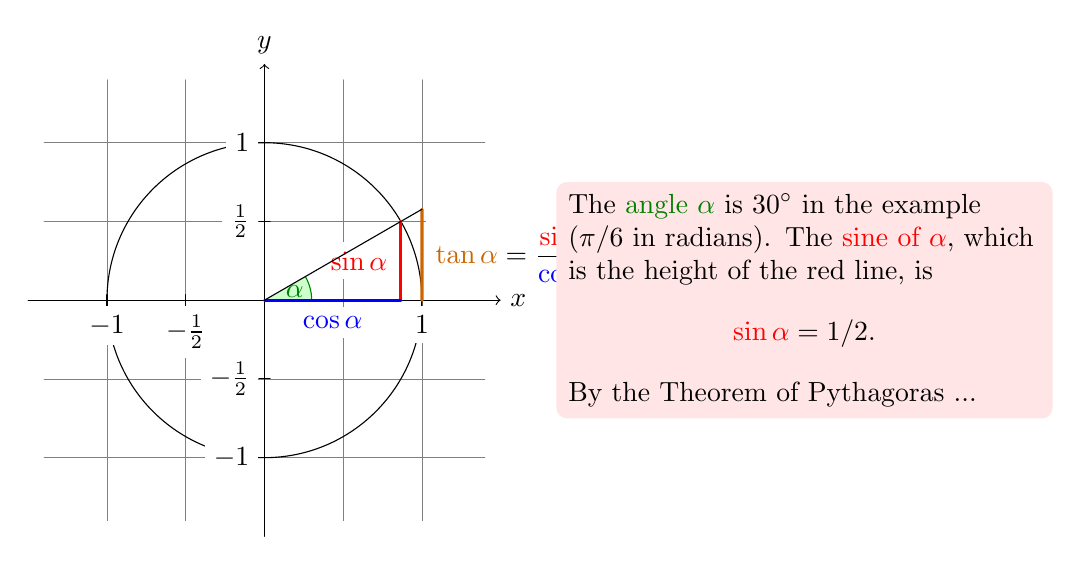
\begin{tikzpicture}[scale=2,cap=round]
  % Local definitions
  \def\costhirty{0.8660256}

  % Colors
  \colorlet{anglecolor}{green!50!black}
  \colorlet{sincolor}{red}
  \colorlet{tancolor}{orange!80!black}
  \colorlet{coscolor}{blue}

  % Styles
  \tikzstyle{axes}=[]
  \tikzstyle{important line}=[very thick]
  \tikzstyle{information text}=[rounded corners,fill=red!10,inner sep=1ex]

  % The graphic
  \draw[style=help lines,step=0.5cm] (-1.4,-1.4) grid (1.4,1.4);
  
  \draw (0,0) circle (1cm);

  \begin{scope}[style=axes]
    \draw[->] (-1.5,0) -- (1.5,0) node[right] {$x$} coordinate(x axis);
    \draw[->] (0,-1.5) -- (0,1.5) node[above] {$y$} coordinate(y axis);

    \foreach \x/\xtext in {-1, -.5/-\frac{1}{2}, 1}
      \draw[xshift=\x cm] (0pt,1pt) -- (0pt,-1pt) node[below,fill=white] {$\xtext$};
  
    \foreach \y/\ytext in {-1, -.5/-\frac{1}{2}, .5/\frac{1}{2}, 1}
      \draw[yshift=\y cm] (1pt,0pt) -- (-1pt,0pt) node[left,fill=white] {$\ytext$};
  \end{scope}
    
  \filldraw[fill=green!20,draw=anglecolor] (0,0) -- (3mm,0pt) arc(0:30:3mm);
  \draw (15:2mm) node[anglecolor] {$\alpha$};
    
  \draw[style=important line,sincolor]
    (30:1cm) -- node[left=1pt,fill=white] {$\sin \alpha$} (30:1cm |- x axis);
  
  \draw[style=important line,coscolor]
    (30:1cm |- x axis) -- node[below=2pt,fill=white] {$\cos \alpha$} (0,0);
  
  \draw[style=important line,tancolor] (1,0) -- node[right=1pt,fill=white] {
    $\displaystyle \tan \alpha \color{black}=
    \frac{{\color{sincolor}\sin \alpha}}{\color{coscolor}\cos \alpha}$}
    (intersection of 0,0--30:1cm and 1,0--1,1) coordinate (t);

  \draw (0,0) -- (t);
  
  \draw[xshift=1.85cm]
    node[right,text width=6cm,style=information text]
    {
      The {\color{anglecolor} angle $\alpha$} is $30^\circ$ in the
      example ($\pi/6$ in radians). The {\color{sincolor}sine of
        $\alpha$}, which is the height of the red line, is
      \[
      {\color{sincolor} \sin \alpha} = 1/2.
      \]
      By the Theorem of Pythagoras ...
    };
\end{tikzpicture}
\caption[A pgf/Tikz drawing]{A drawing taken from the pgf
  manual/tutorial by Till Tantau}
\label{fig:tikz}
\end{figure}


%%% Local Variables: 
%%% mode: latex
%%% TeX-master: "main"
%%% End: 
